\documentclass{article}
\usepackage{tikz}
\usetikzlibrary{bayesnet}

\begin{document}

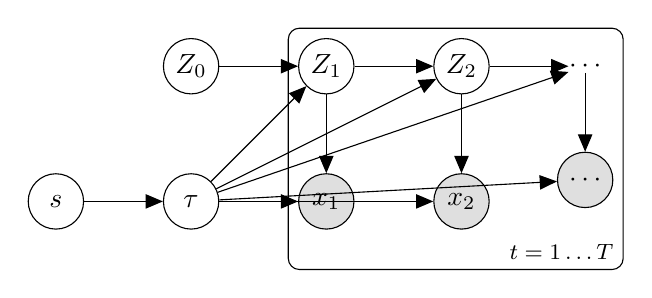
\begin{tikzpicture}
  % Nodes
  \node[latent]                                (s) {$s$};
  \node[latent, right=of s]                    (tau) {$\tau$};
  \node[latent, above=of tau]                  (z0) {$Z_0$};
  \node[latent, right=of z0]                   (z1) {$Z_1$};
  \node[latent, right=of z1]                   (z2) {$Z_2$};
  \node[obs, below=of z1]                      (x1) {$x_1$};
  \node[obs, below=of z2]                      (x2) {$x_2$};
  \node[const, right=of z2]                    (zT) {$\cdots$};
  \node[obs, below=of zT]                      (xT) {$\cdots$};

  % Edges
  \edge {s} {tau};
  \edge {tau} {z1, z2, zT}; % tau influences all Z from Z_1 onwards
  \edge {z0} {z1}; % Transition from Z_0 to Z_1
  \edge {z1} {z2}; % Transition from Z_1 to Z_2
  \edge {z2} {zT}; % Transition to more Z_t
  \edge {tau,z1} {x1}; % Dependence of x_1 on Z_1 and tau
  \edge {tau,z2} {x2}; % Dependence of x_2 on Z_2 and tau
  \edge {tau,zT} {xT}; % Dependence of future x_t on Z_t and tau

  % Plates
  \plate {time} {(z1)(z2)(zT)(x1)(x2)(xT)} {$t = 1 \ldots T$};
\end{tikzpicture}

\end{document}
